\documentclass[11pt,a4paper]{article}

\usepackage[english]{babel}
\usepackage[T1]{fontenc}
\usepackage[utf8]{inputenc}
\usepackage{graphicx}
\graphicspath{{../Figs/}}
\usepackage{float}
\usepackage{subcaption}
\usepackage[font=footnotesize,labelfont={sf,bf},textfont=sf,width=\textwidth]{caption}
\usepackage[margin=2cm]{geometry}
\usepackage[plainpages=false,pdfpagelabels,hypertexnames=false]{hyperref}
\usepackage[usenames,dvipsnames]{xcolor}
\usepackage{mathtools}
\usepackage[separate-uncertainty=true, multi-part-units=single]{siunitx}
\usepackage{booktabs}
\usepackage{physics}
\usepackage[title]{appendix}

\title{\bfseries\textsc{Hall effect in semiconductors}}
\author{
Michele Masini\\ \small\texttt{\href{mailto:michele.masini@uni-ulm.de}{michele.masini@uni-ulm.de}}\and
Iyán Méndez Veiga\\ \small\texttt{\href{mailto:iyan.mendez-veiga@uni-ulm.de}{iyan.mendez-veiga@uni-ulm.de}}
}
\date{\today}

\begin{document}
\maketitle

\section{Introduction}
In this experiment, we determine the carrier density ($p$) and the mobility ($\mu$) of a p-type Silicon semiconducting sample doped with Boron. We determine these quantities as a function of the temperature in the range \SIrange{80}{300}{\kelvin}.

In order to obtain the carrier density we use the Hall effect. Once the Hall coefficient is known, mobility is computed by measuring the resistivity ($\rho$) of the sample. Since preparing a «Hall bar» is very time consuming, resistivity is measured by means of the van der Pauw method.

\section{Theory}

\subsection{Carrier density}
Let us start explaining the evaluation of the carrier density.

Our sample is under the influence a constant magnetic field ($\vec{B}$). We can evaluate the drift velocity ($\vec{v}_d$) its charge carriers using the equations of motion of a particle in presence of an electric field:
\begin{equation*}
m\frac{d\vec{v}}{dt}+\frac{m}{\tau}\vec{v}_d=-e(\vec{E}+\vec{v}\times\vec{B})
\end{equation*}
where $\tau$ is called relaxation time and in a microscopic picture it describes the mean time between two successive collision. The steady state solution of this equation is: 
\begin{equation*}
\vec{v}_d=-\frac{e\tau}{m}(\vec{E}+\vec{v}_d\times\vec{B})\equiv -\mu (\vec{E}+\vec{v}_d\times\vec{B})\,,
\end{equation*}
where we have defined the \emph{mobility} $\mu$.
%In our case the electric field will be parallel to the surface of the sample and the magnetic field orthogonal, hence we can remove the vectors.

Using the definition of current density in a p-doped material:
\begin{equation*}
\vec{j}=ep\vec{v}_d\,,
\end{equation*}
where $e$ is the elementary charge and $p$ is the holes density, we get the following expression for the electric field:
\begin{equation*}
\vec{E}=\frac{1}{ep\mu}\vec{j}+\frac{1}{ep}\vec{j}\times\vec{B}\equiv \vec{E}_\parallel+\vec{E}_\perp
\end{equation*}

Therefore, by measuring the voltage between two random points P and N of the sample (as shown in figure ({\color{red}Ref figure}), we obtain:
\begin{equation}\label{eq:U_PN}
U_\text{PN}=\int_P^N\vec{E}\cdot d\vec{s}=\int_P^{N'}\vec{E}_\perp\cdot d\vec{s}+\int_{N'}^N\vec{E}_\parallel\cdot d\vec{s}
\end{equation}
We call the second term in \eqref{eq:U_PN} \emph{offset voltage} ($U_\text{off}$). This term can be measured in absence of magnetic field. The first term can be evaluated considering that the magnetic field is orthogonal to the sample surface:
\begin{equation}
\int_P^{N'}\vec{E}_\perp\cdot d\vec{s}=-\frac{B}{ep}\int_P^{N'}j\, ds=-\frac{B}{ep}\int_P^{N'}\frac{1}{d}\frac{dI}{ds}\, ds=-\frac{B}{epd}\int_P^{N'} dI=-\frac{BI}{epd}
\end{equation}
Defining $R_H\equiv\dfrac{1}{ep}$ as the Hall coefficient, we get the relation that will allow us to measure the carrier density:
\begin{equation}\label{eq:Hall_voltage}
U_\text{PN}-U_\text{off}=-R_H\frac{BI}{d}\,,
\end{equation}
when $B$ and $I$ are fixed and the sample's thickness $d$ is known.

\subsection{Dependence of $p$ on the temperature}

In a semiconductor, the occupation of electronic states follows the Fermi-Dirac distribution:
\begin{equation*}
f(E,T)=\frac{1}{1+e^{\frac{E-E_F}{k_BT}}}
\end{equation*}
Since in our case the charge carriers are holes, our distribution will be $1-f(E,T)$. Let us call $D_V(E)$ the density of states in the valence band and $E_V$ the valence band edge, then we can write the carriers density as:
\begin{equation}
p=\int_{-\infty}^{E_V}D_V(E)(1-f(E,T))dE
\end{equation}
The density of states can be written according to the parabolic approximation:
\begin{equation*}
D_V(E)=\frac{\sqrt{2}(m_{lh}^{3/2}+m_{hh}^{3/2})}{2\pi^2\hbar^3}\sqrt{E_V-E}
\end{equation*} where $m_{lh}$ and $m_{hh}$ are the mass of light and heavy holes.

Finally, defining 
\begin{equation}
N_V=2\frac{(m_{lh}^{3/2}+m_{hh}^{3/2})}{h^3}(2\pi k_BT)^{3/2}
\end{equation} we can write the following formula for the carriers density:
\begin{equation}
p=N_V\frac{2}{\sqrt{\pi}}F_{1/2}\left(\frac{E_V-E_F}{k_BT}\right)
\end{equation} where $F_{1/2}(y)=\int_0^\infty\frac{x^{1/2}}{1+e^{(x-y)}}dx$ is the Fermi-Dirac integral and $E_F$ is the Fermi energy. In the case $k_BT<<E_F-E_V$ the solution of the integral is:
\begin{equation}
p=N_Ve^{-\frac{E_F-E_V}{k_BT}}\label{eq::p}
\end{equation}

In our case the semiconductor is p-doped, i.e. a concentration $N_A$ of electrons acceptors has been artificially added to the material. We can express the concentration of ionized acceptors as:
\begin{equation}
N_A^-=\frac{N_A}{1+4e^{\frac{E_A-E_F}{k_BT}}}\label{eq::Na-}
\end{equation}
here $E_A$ is the energy of bound acceptor holes.

The matierial needs to respect the neutrality of charge, i.e. $p=n+N_A^-$. The intrinsic conductivity is neglectable for a certain range of temperatures, in this case we can write the charge neutrality as $p=N_A^-$. Hence, using Eqs.~(\ref{eq::Na-}),~(\ref{eq::p}) we obtain:
\begin{equation}
p\simeq\frac{N_A}{1+4(p/N_V)e^{\frac{E_A-E_V}{k_BT}}}
\end{equation}
Solving the equation for $p$, we get:
\begin{equation}
p=\simeq\frac{2N_A}{1+\sqrt{1+16\frac{N_A}{N_V}e^\frac{E_A-E_V}{k_BT}}}
\end{equation}For low temperatures ($T<<\frac{E_A-E_V}{k_B}$) we can simplify the previous expression as:
\begin{equation}
p\simeq \frac{1}{2}\sqrt{N_AN_V}e^{-\frac{E_A-E_V}{2K_BT}}
\end{equation}

\subsection{Mobility}
At this point we will use Van der Pauw method to get the mobility. In 1958 this author \cite{vdP} proved that if we apply a voltage putting sufficently small conctacts at the border of our sample, the sample is homogeneous in thickness ($d$) and it has no isolated holes, then the following formula holds:
\begin{equation}
e^{-\frac{\pi R_{AB,CD}d}{\rho}}+e^{-\frac{\pi R_{BC,DA}d}{\rho}}=1
\end{equation}
where $\rho$ is the resistivity, while $R_{AB,CD}$ is defined as the ratio between the voltage applied between the contact points C and D and the current measured between the points A and B and $R_{BC,DA}$ analogously.

As shown in the paper, we can get the resistivity according to the following expression:
\begin{equation}
\rho=\frac{\pi d}{\ln(2)}\frac{(R_{AB,CD}+R_{BC,DA})}{2}f\left(R_{AB,CD},R_{BC,DA}\right)
\end{equation}
where the function $f$ can be approximated as
\begin{equation}
f \simeq 1-\left(\frac{R_{AB,CD}-R_{BC,DA}}{R_{AB,CD}+R_{BC,DA}}\right)^2 \frac{\ln(2)}{2}-\left(\frac{R_{AB,CD}-R_{BC,DA}}{R_{AB,CD}+R_{BC,DA}}\right)^4\left(\frac{\ln(2)^2}{4}-\frac{\ln(2)^3}{12}\right)
\end{equation}

%Now we will show how to use the resistivity in order to get the mobility. Let us consider a magnetic field $B_z$ orthogonal to the surface of our sample of thickness $d$ and largeness $L$. {\large (need a picture)} In the steady state, the force along y-direction is zero:
%\begin{equation*}
%e(-E_y+v_xB_z)=0 \Rightarrow v_x=E_y/B_z
%\end{equation*}
%In this condition the current is only along x and is given by $I=pev_xLd$. Using the definition of Hall coefficient seen before, we obtain
%\begin{equation}
%R_H=\frac{1}{ep}=\frac{v_xLd}{I}=\frac{E_yLd}{B_zI}
%\end{equation}
%Since the voltage is $V=E_yL$ we can write $R_H=\frac{Vd}{B_zI}$. Finally, using the fact that $\rho=R_H/\mu$, we obtain our expression:
In order to evaluate the mobility we will use the following expression:
\begin{equation}
\mu=\frac{d}{B}\frac{R_H}{\rho}
\end{equation}

\section{Materials and methods}

The experimental setup consisted in a liquid nitrogen cryostat DN1710 by Oxford Instruments Ltd. surrounded at the bottom by an electromagnet Bruker Magnet B-E 10 (see Figure \ref{fig:experimental_setup_all}).

Sample was connected to a HP 34401A Digital Multimeter and a Yokogawa 7651 Programmable DC Source. In order to select to which sample contacts they were connected, device shown in Figure \ref{fig:cables} was used.

\begin{figure}[H]
\centering
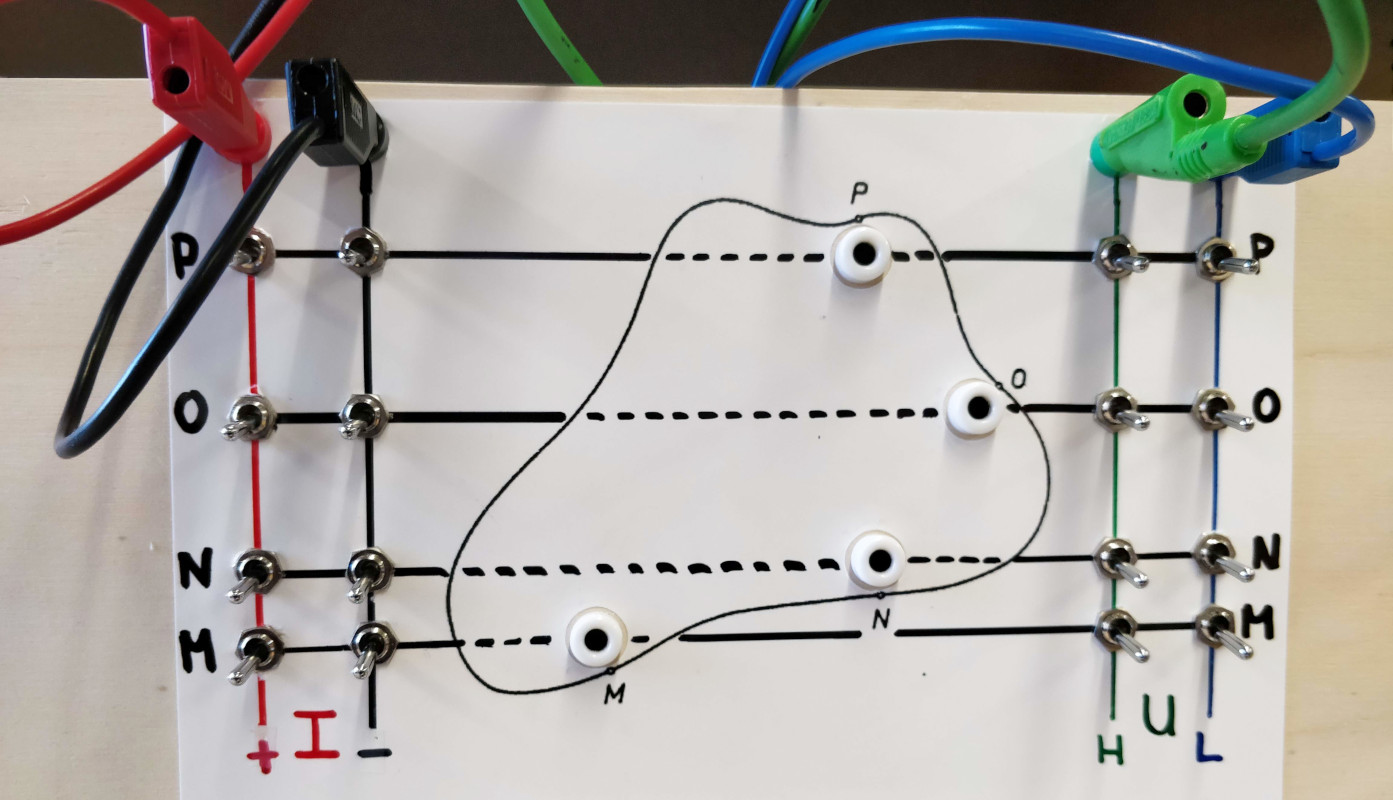
\includegraphics[width=0.6\textwidth]{Experimental_setup_cables}
\caption{Device to choose where to apply current in the semiconductor sample and where to measure voltage. For example, by turning on switches M and O on the left (current), and switches P and N on the right (voltages), we can measure the transvere voltage $U_t$.}
\label{fig:cables}
\end{figure}

For the characterization of the magnetic field, a calibrated Hall sensor (see Figure \ref{fig:Hall_sensor}) was used connected to the probe tube.

\begin{figure}[H]
\centering
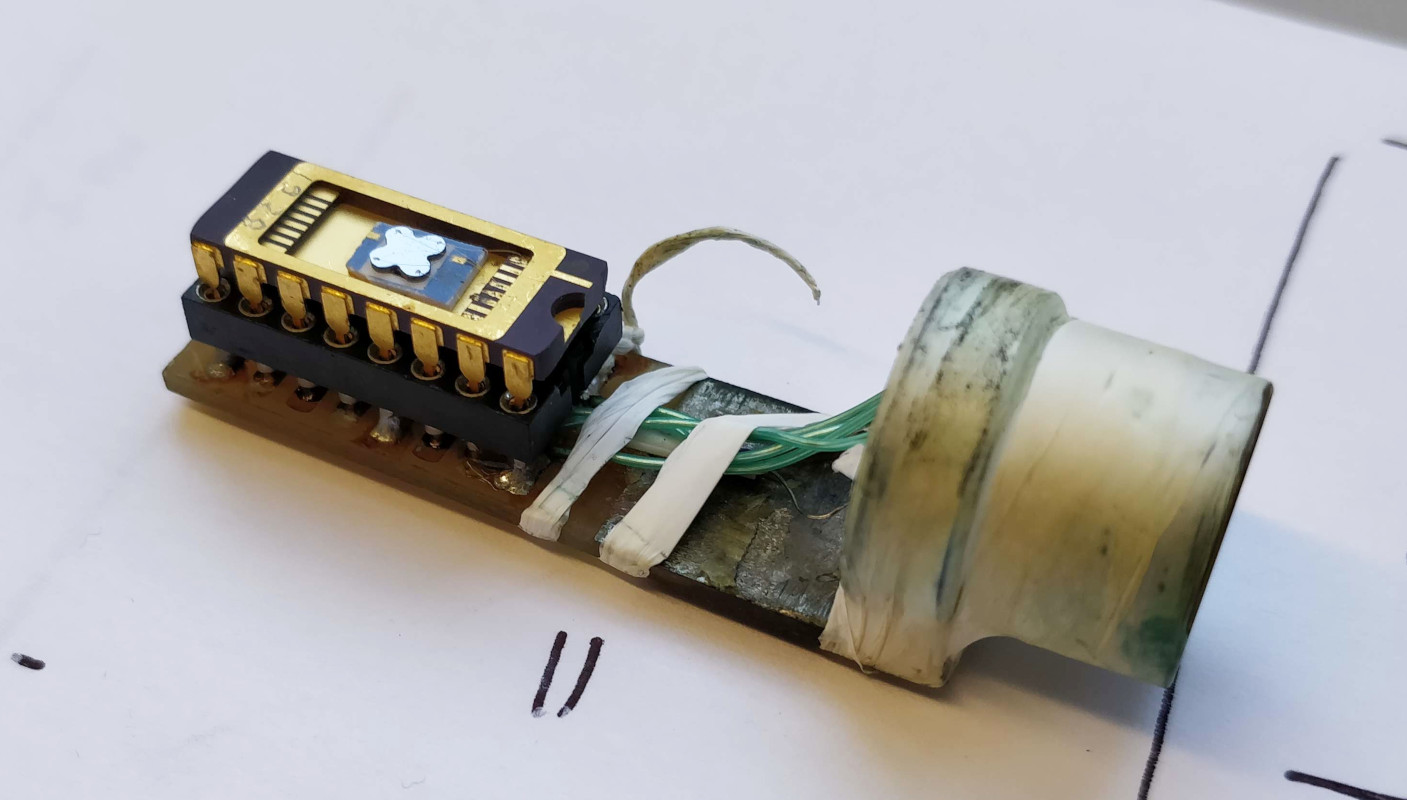
\includegraphics[width=0.6\textwidth]{Hall_sensor}
\caption{Calibrated Hall sensor (\SI{0.1172}{\tesla/\milli\volt} at \SI{10}{\milli\ampere}) used to measure the magnetic field produced by the coils.}
\label{fig:Hall_sensor}
\end{figure}

Finally, determination of the temperature close to the sample was done with a resistor connected to a device that directly show us the temperature in Kelvin (see Figure \ref{fig:temperature_device}). With the same device, we could control a heating mechanism by applying a voltage to a different resistor in the cryostat.

\begin{figure}[H]
\centering
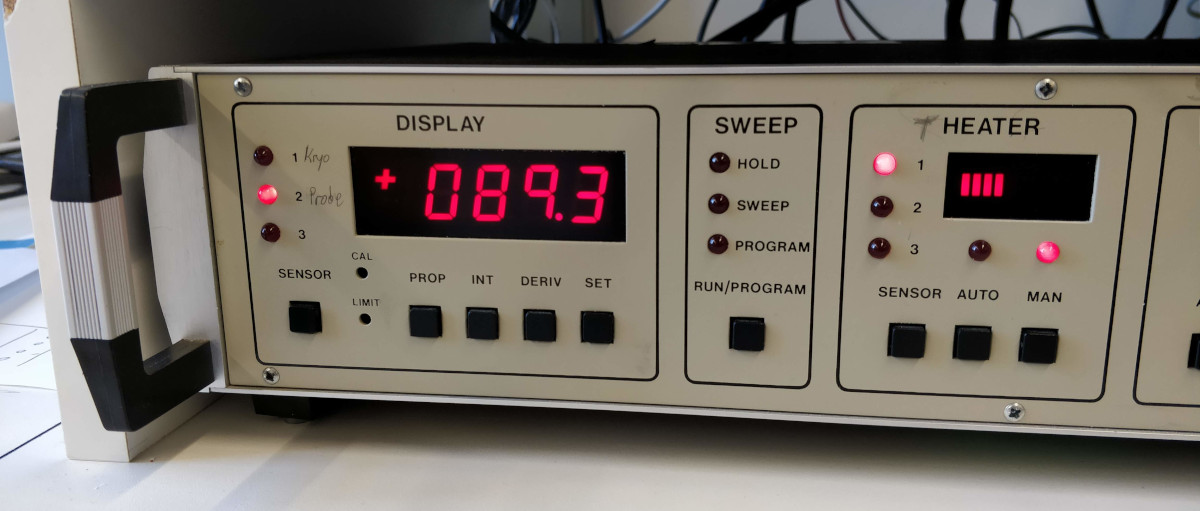
\includegraphics[width=0.6\textwidth]{temperature_device}
\caption{Device showing that temperature close to the sample is \SI{89.3}{\kelvin}. A voltage of \SI{8}{\volt} was being used at that moment to heat the sample after closing the gas exhaust valve.}
\label{fig:temperature_device}
\end{figure}

\begin{figure}[H]
\centering
\begin{subfigure}[b]{0.45\textwidth}
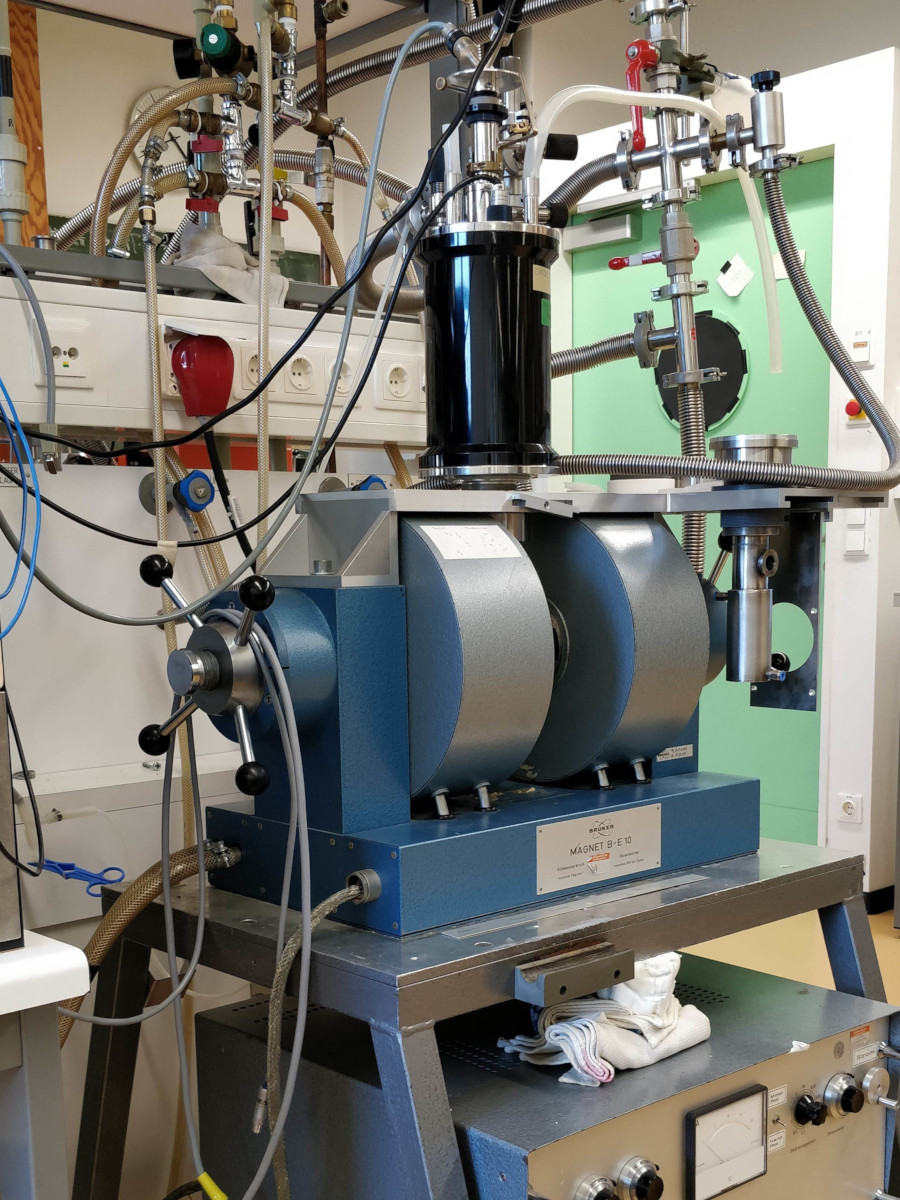
\includegraphics[width=\textwidth]{Experimental_setup}
\caption{}
\label{fig:experimental_setup}
\end{subfigure}
\begin{subfigure}[b]{0.45\textwidth}
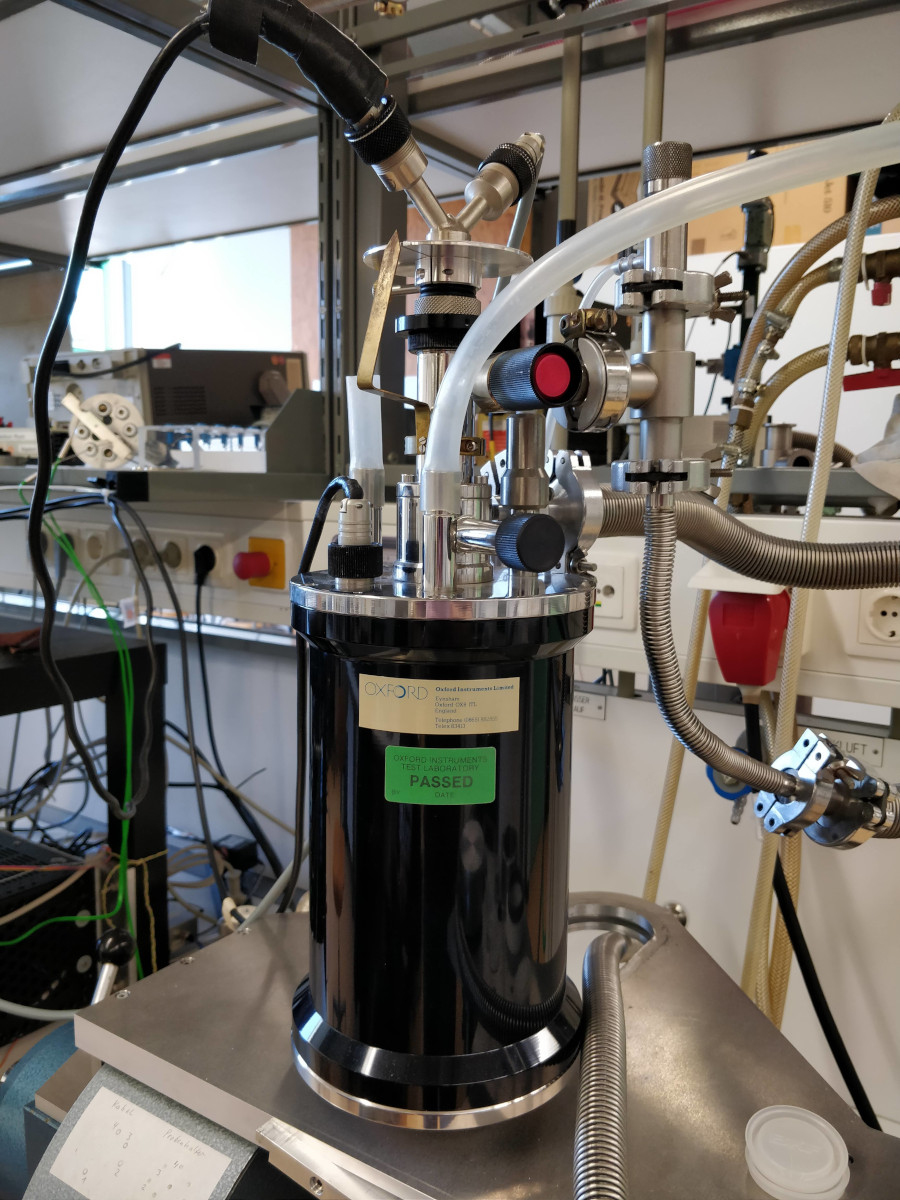
\includegraphics[width=\textwidth]{cryostat}
\caption{}
\label{fig:cryostat}
\end{subfigure}\\\vspace{.2cm}
\begin{subfigure}[b]{0.6\textwidth}
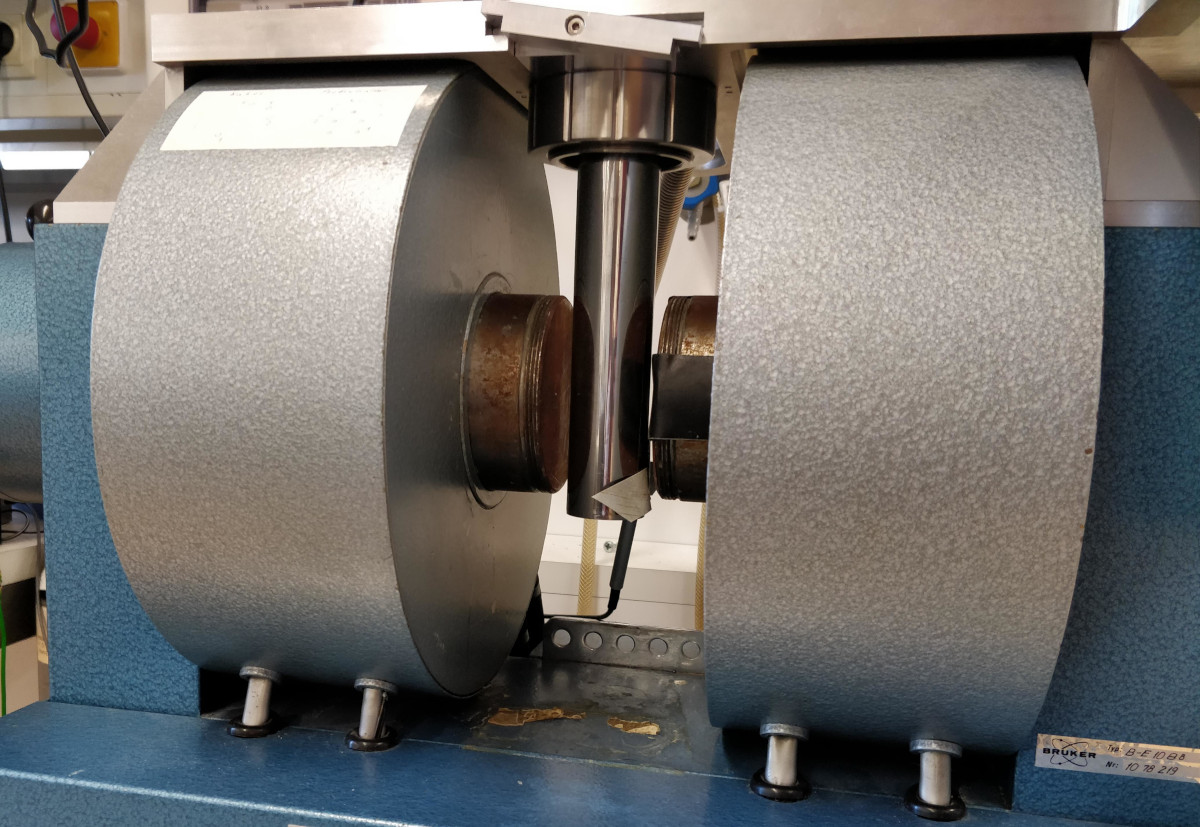
\includegraphics[width=\textwidth]{electromagnet}
\caption{}
\label{fig:electromagnet}
\end{subfigure}
\caption{Experimental setup used for this experiment. In (a) the cryostat with the bottom, where the sample is placed, enclosed by the magnetic coils. In (b) the cryostat in more detail. Transparent tube in the center is connected to a vacuum pump. Left one is the nitrogen entry port. Black valve in the center is the gas exhaust valve. By closing it, temperature starts to rise. Sample is introduced using a probe tube in the sample access port at the top centre. In both (a) and (b) probe tube is already introduced and the cables connected to sample's contacts can be seen, as well as tip to determine the angle between sample and magnetic field. In (c) the electromagnet in detail.}
\label{fig:experimental_setup_all}
\end{figure}



\section{Results and discussion}

\subsection{Calibration of the electromagnet}

We determined the dependence of the magnetic field strength $B$ on the current $I_B$ through the magnetic coils using a calibrated Hall sensor (see Figure \ref{fig:Hall_sensor}).

We measured the voltage for different currents $I_B$ from \SI{0}{\ampere} to \SI{15}{\ampere} in steps of \SI{1}{\ampere} at room temperature ($\sim\SI{300}{\kelvin}$). In Figure \ref{fig:magnetic_field}, the magnetic field computed using the calibration coefficient (see caption Figure \ref{fig:Hall_sensor}) is plotted against the current $I_B$.

\begin{figure}[H]
\centering
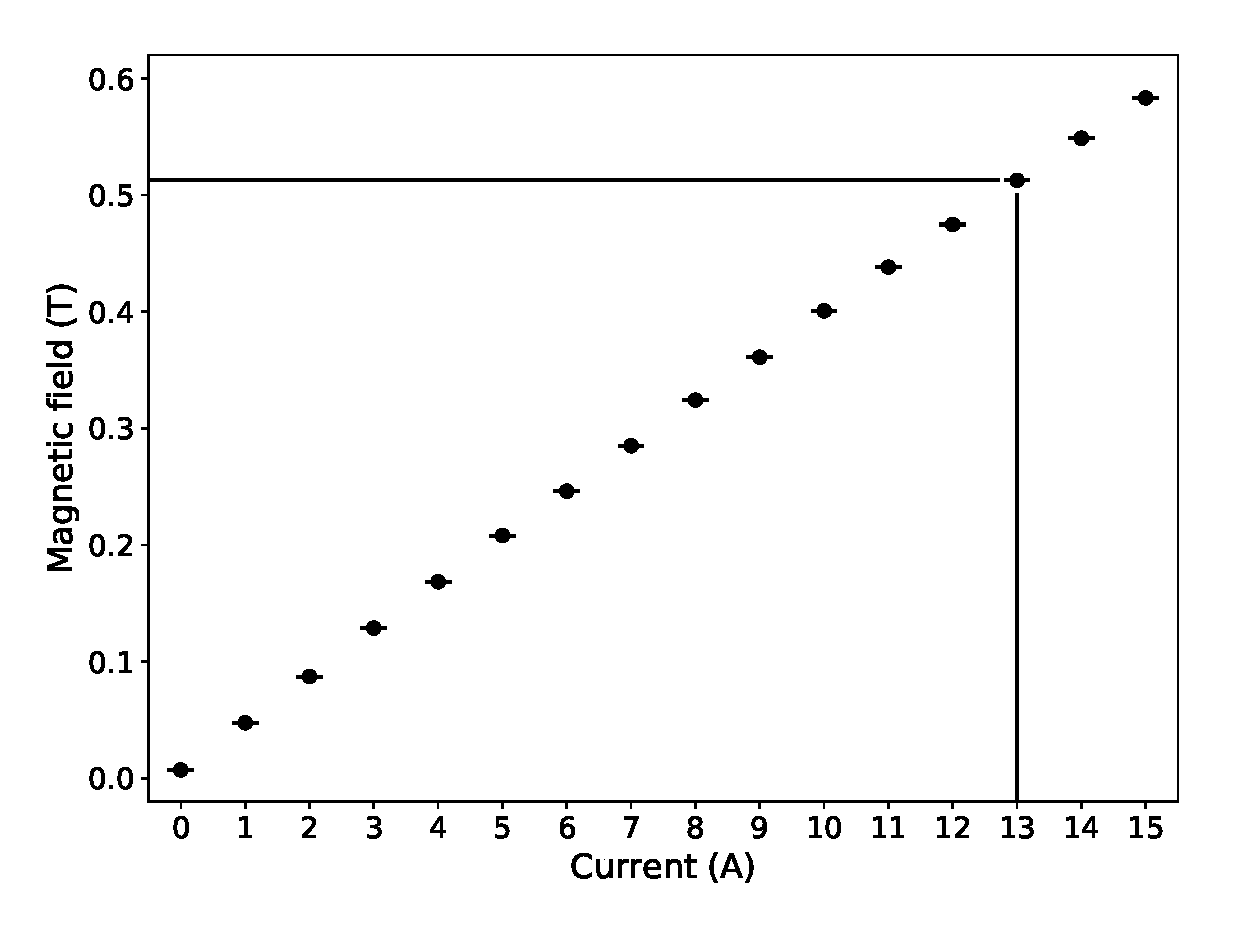
\includegraphics[width=0.8\textwidth]{Magnetic_field_vs_current.eps}
\caption{Magnetic field vs current in the magnetic coils. Solid lines show the current we fixed in the coils for the following measurements, generating a magnetic field of \SI{0.5126}{\tesla}.}
\label{fig:magnetic_field}
\end{figure}

\subsection{Checking ohmic behaviour}

The junction between conductors should have a linear current-voltage curve. We checked this by measuring the voltage between two points for currents from \SI{0}{\micro\ampere} to \SI{150}{\micro\ampere} in steps of \SI{10}{\micro\ampere} also at room temperature. In Figure \ref{fig:ohmic_check}, the linear behaviour is clearly showed.

\begin{figure}[H]
\centering
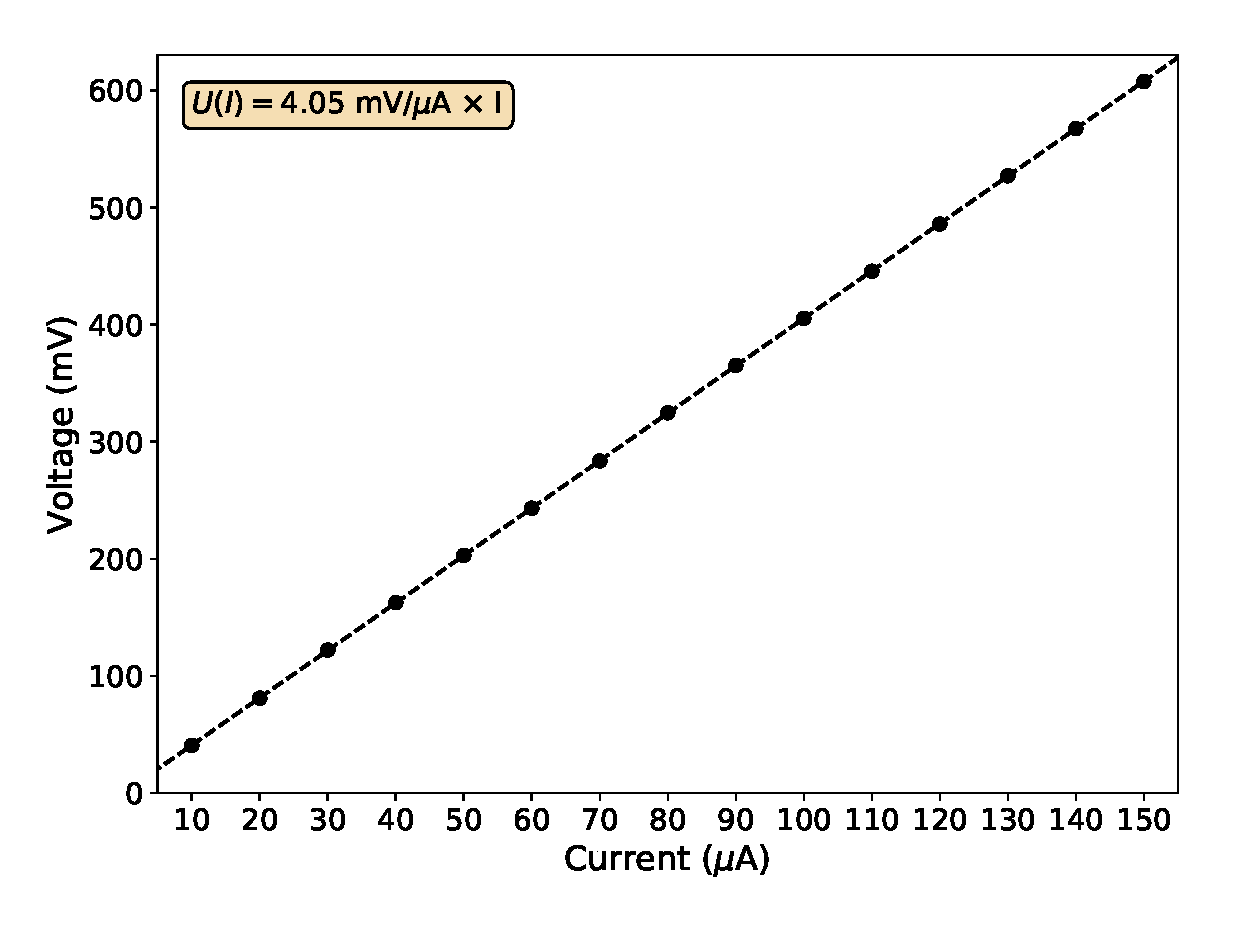
\includegraphics[width=0.8\textwidth]{Voltage_vs_current_ohmic_test.eps}
\caption{Measured voltage vs applied current between two sample contacts. The dashed line is a linear fit of the experimental data with slope \SI{4.05}{\milli\volt/\milli\ampere}.}
\label{fig:ohmic_check}
\end{figure}

\subsection{Orientation of the sample}

In order to align the sample perpendicular to the magnetic field generated by the coils, we measured the transverse voltage $U_t$, i.e. the Hall voltage plus the offset voltage (see {\color{red}Reference theory or figure}), with a fixed magnetic field $B=\SI{0.5126}{\tesla}$ and current $I=\SI{100}{\micro\ampere}$ for different angles between the magnetic field and the surface normal of the sample from \ang{-90} to \ang{90} in steps of \ang{10}.

\begin{figure}[H]
\centering
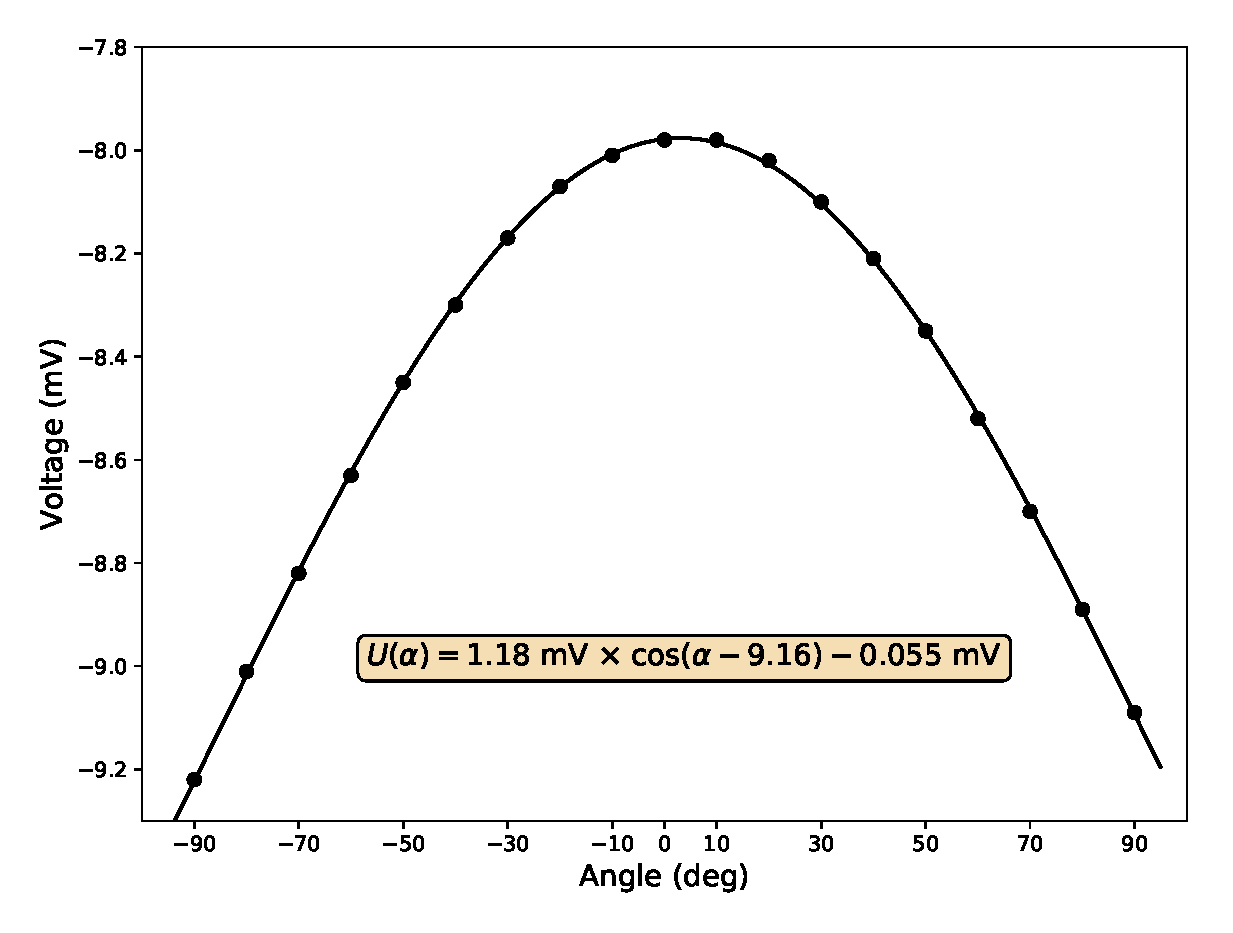
\includegraphics[width=0.8\textwidth]{Voltage_vs_angle.eps}
\caption{Transverse voltage vs orientation angle of the sample with respect to the applied magnetic field. Dash line is a fit using the function $U_t(\alpha)=U_0\cos(\alpha+\phi) + U_\text{off}$. Values obtained for the fitting parameters are shown in the plot box.}
\label{fig:orientation}
\end{figure}

\subsection{Determination of $p$ and $\mu$}

After the calibration measurements, we cooled down the sample to about \SI{80}{\kelvin} using liquid nitrogen. At a temperature of \SI{82}{\kelvin} we started to do the following measurements every \SI{5}{\kelvin} while warming up the sample applying a voltage to a resistor in the cryostat. Temperature was measured by a different resistor close to the sample.
\begin{itemize}
\item Offset voltage $U_\text{off}$, i.e. the potential difference between contacts P and N (see Figure {\color{red}Add figure with experimental setup to change currents and measure voltages}), while applying a current of \SI{100}{\micro\ampere} between contacts M and O and without magnetic field.
\item Transverse voltage $U_t$ between contacts P and N, i.e. the sum of Hall voltage and the offset voltage, while applying same current of \SI{100}{\micro\ampere} between M and O and with a magnetic field of \SI{0.5126}{\tesla}.
\item The potential difference $U_\text{OP}$ between contacts O and P while applying a current of \SI{100}{\micro\ampere} between contacts M and N and with the same magnetic field as before.
\item The potential difference $U_\text{PM}$ between contacts P and M while applying the same current between contacts N and O and under the same magnetic field.
\end{itemize}

First two measurements are used to compute the Hall constant $R_H$ and the carrier concentration $p$ of our p-doped semiconductor. The other two are necessary to obtain the resistivity $\rho$ using the van der Pauw method \cite{vdP}. Once $R_H$ and $\rho$ are known, it is also possible to compute the Hall mobility $\mu_H$.

We were able to measure these four values from \SI{82}{\kelvin} to \SI{200}{\kelvin}, but heating process was too slow to reach \SI{300}{\kelvin} so we were given measurements from other group. We combined theirs with ours to get the full range of temperatures (see Appendix \ref{app:dataset}).

\section{Conclusions}

\nocite{*}
\vfill
\bibliographystyle{unsrt}
\bibliography{references}

\newpage
\begin{appendices}
\section{Joining measurements}\label{app:dataset}
Due to a problem with the heating mechanism in the cryostat, we could only do measurements from \SI{82}{\kelvin} to \SI{200}{\kelvin}. The complete raw data from a different group was given to us so we would have measurements in the range from \SI{80}{\kelvin} to \SI{300}{\kelvin}. In this appendix we compare our measurements at low temperatures with theirs, and we showed how he generate a combined dataset.

In Figure \ref{fig:comparison_datasets} we summarize the comparison of both datasets. There is a good enough agreement between them so we decided to join them together and use our measurements at low temperatures and theirs from \SI{200}{\kelvin} to \SI{300}{\kelvin}. The noticeable deviation at low temperatures may be due to the fact that they aligned the sample at a slightly different angle with the magnetic field. This angle was not included in the their dataset but deviation is negligible at higher temperatures.

\begin{figure}[H]
\centering
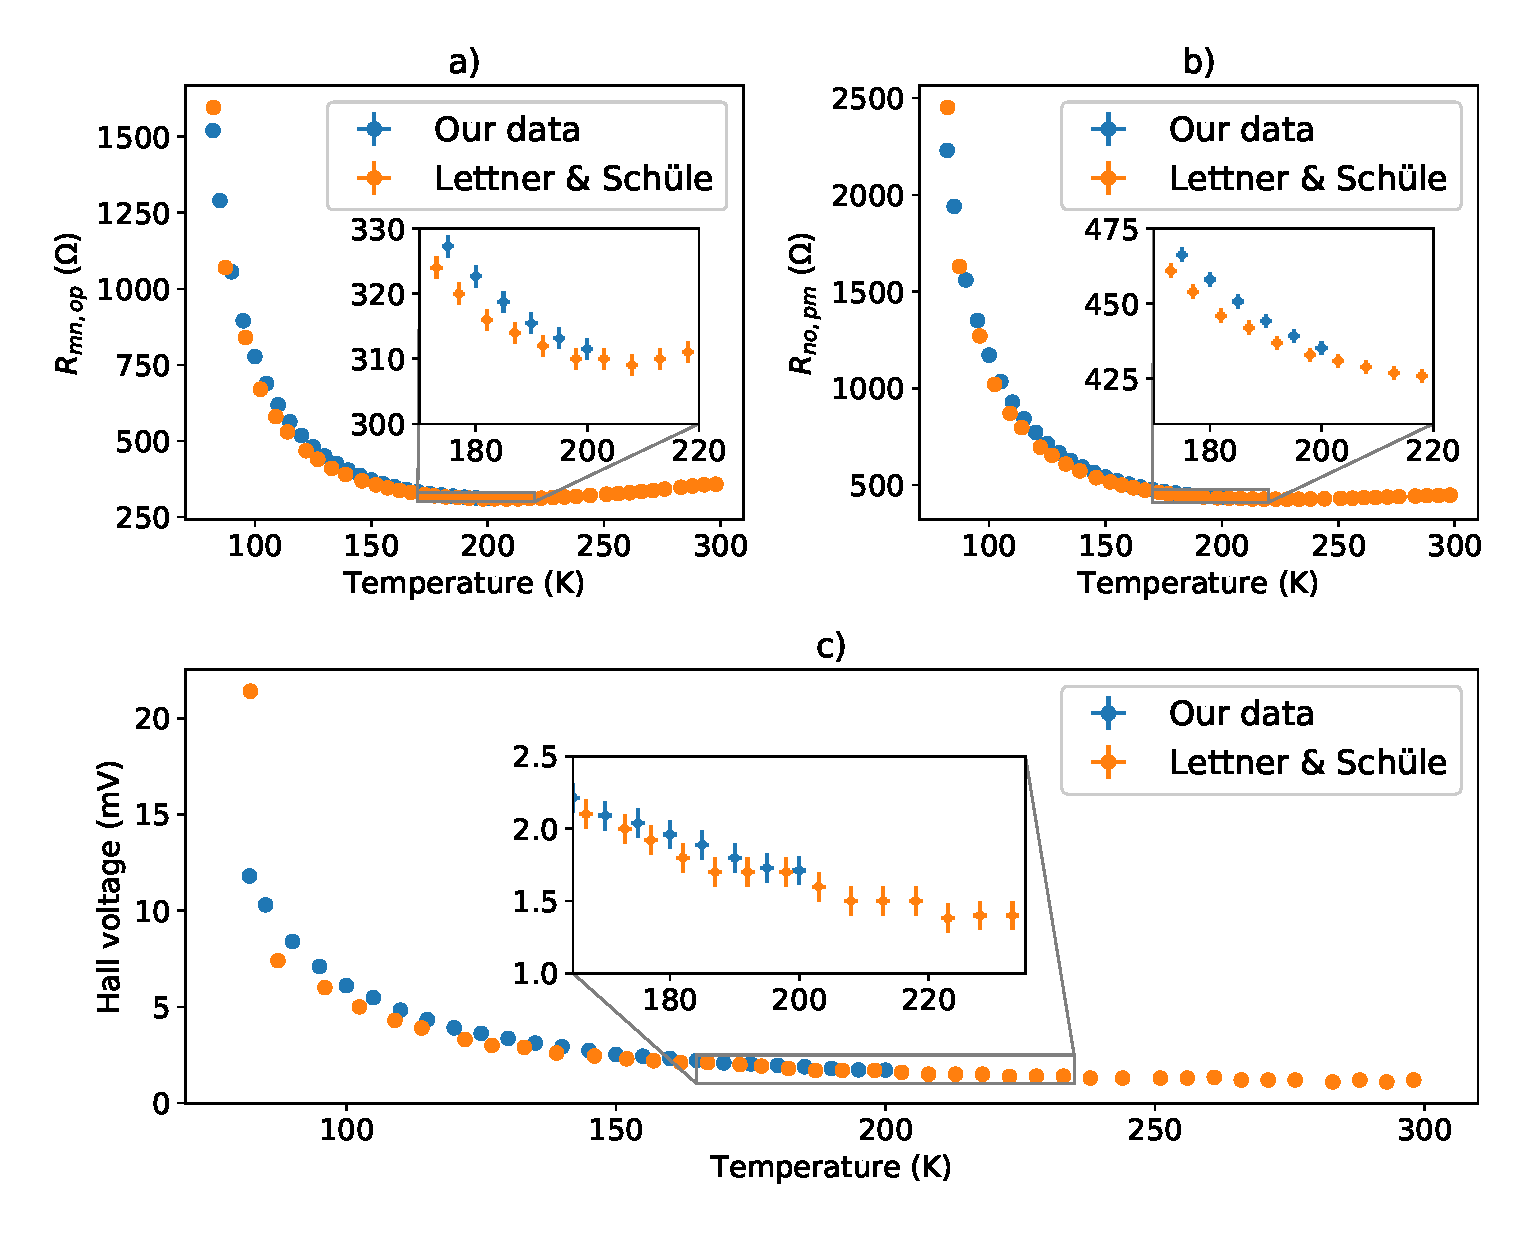
\includegraphics[width=\textwidth]{comparison_datasets.eps}
\caption{In a) and b) the two resistances computed from the measured voltages and in c) the Hall voltage are plotted against temperature. Blue dots represent our measurements and orage dots the values obtained by the other group. Zoomed areas are drawn around $T=\SI{200}{\kelvin}$ to better show the union between our measurements and theirs for our last recorded temperature.}
\label{fig:comparison_datasets}
\end{figure}

Final dataset consists of 25 temperatures from our dataset and 19 from theirs and it is shown in Figure \ref{fig:final_dataset}. All the plots in the report are obtained using this dataset.

\begin{figure}[H]
\centering
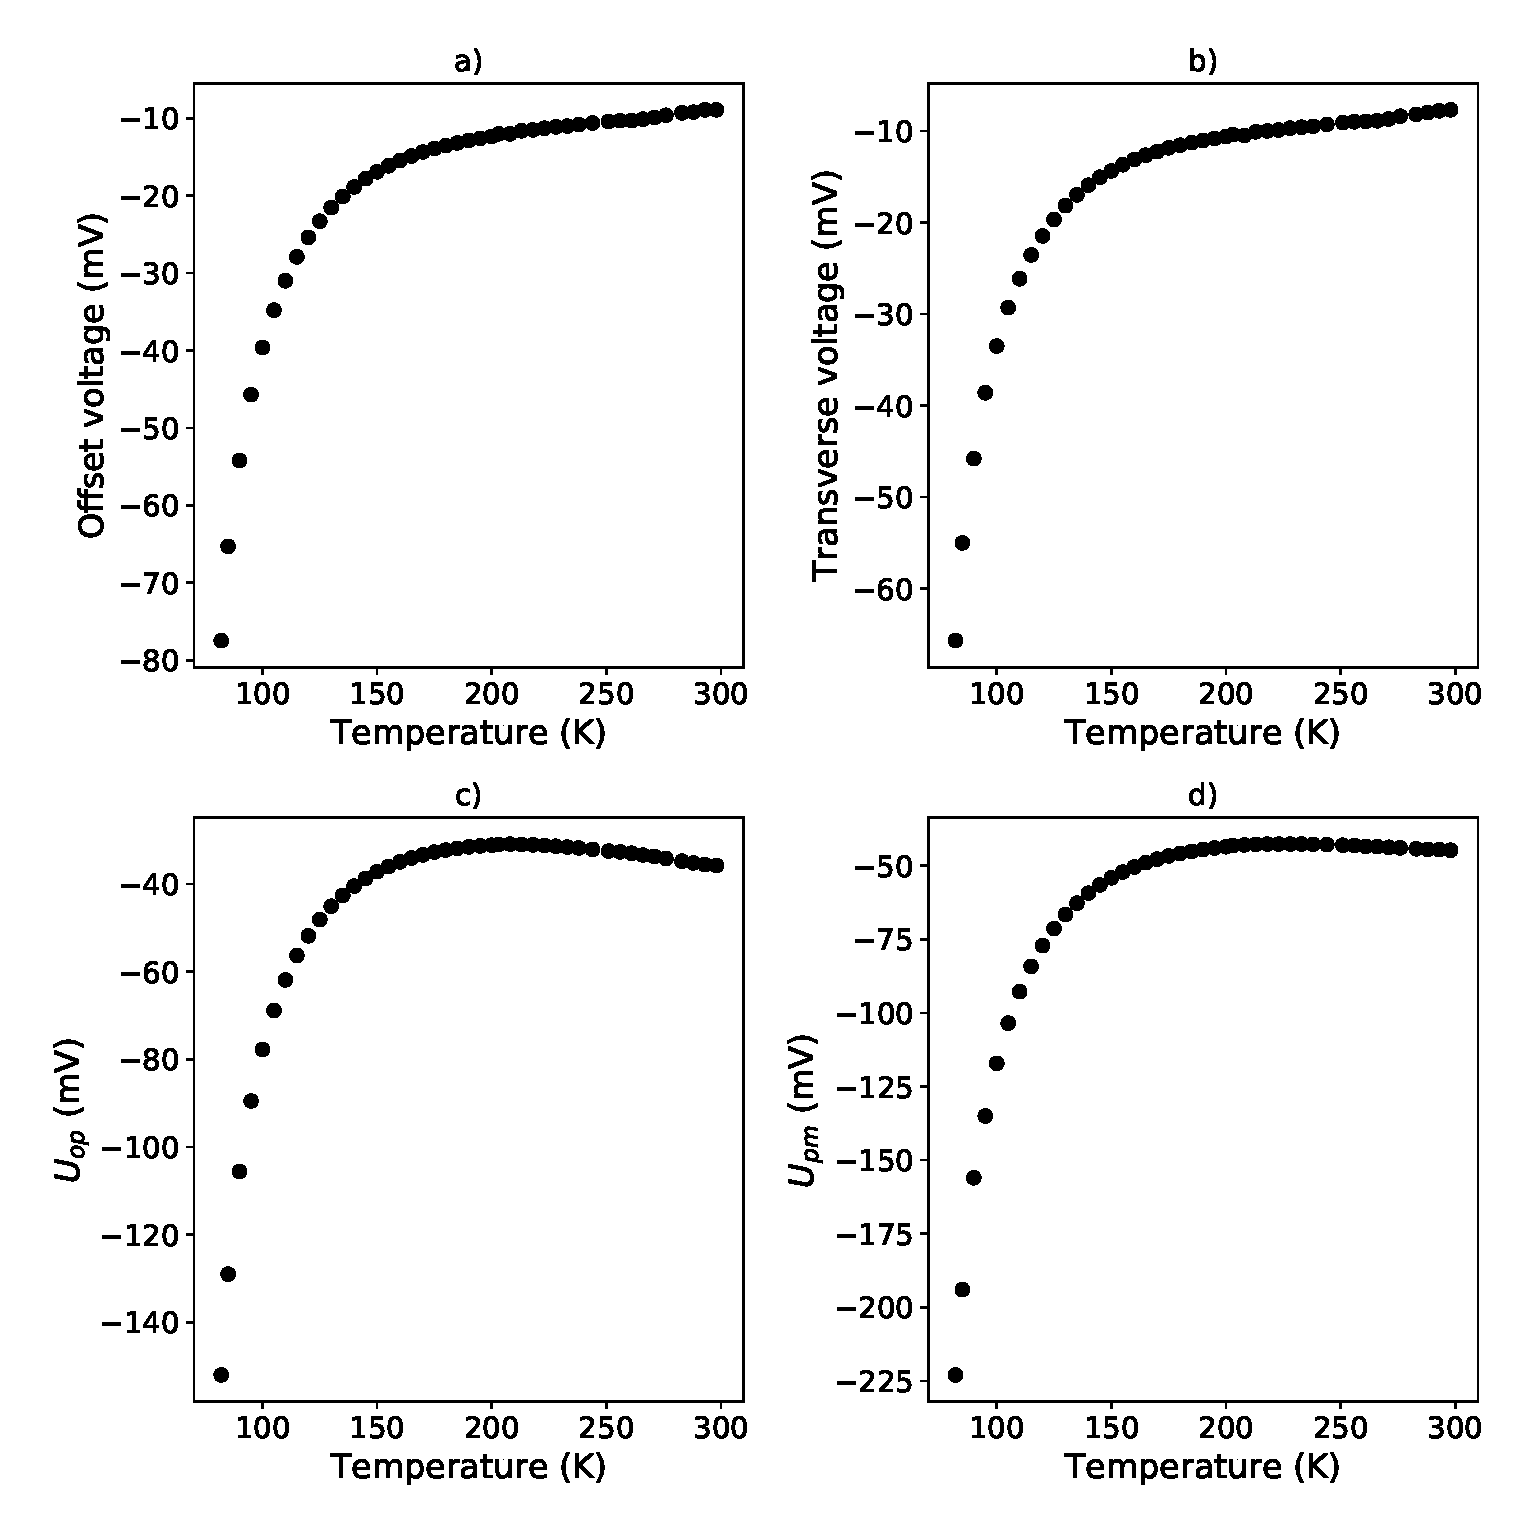
\includegraphics[width=\textwidth]{final_dataset.eps}
\caption{Final dataset with the combined measurements. The four measured quantities in the lab are plotted against the temperature: a) the offset voltage in absence of magnetic field, b) the total transverse voltage and c-d) the two voltages required to use the van der Pauw method.}
\label{fig:final_dataset}
\end{figure}

\end{appendices}

\end{document}